%%%%
\section{Informações sobre a amostragem}

% http://maps.google.com/maps/ms?ie=UTF8&hl=en&msa=0&msid=116003586198857296821.00046d7e7367b947abe12&z=12

A campanha de amostragem ocorreu em Acra (capital de Gana) 
entre 11 de Novembro de 2006 e 15 de Agosto de 2008. 
Foram coletadas 879 amostras de 48 horas no topo de duas residências 
no bairro de \textbf{Nima}.

Os dois pontos de amostragem distam entre si 280 metros, sendo um na rua
\textbf{Sam Rd} com característica residencial
(+5$\degree$ 35$'$ 2$''$,-0$\degree$ 11$'$ 58$''$)
e o outro na avenida \textbf{Al-Waleed bin Talal Highway} 
(+5$\degree$ 34$'$ 54$''$, -0$\degree$ 11$'$ 56.3$''$) com comércios e
alta movimentação veículos, pois conecta diversos bairros ao centro
\ref{fig:nima}. 

\begin{figure}[H]
\begin{center}
  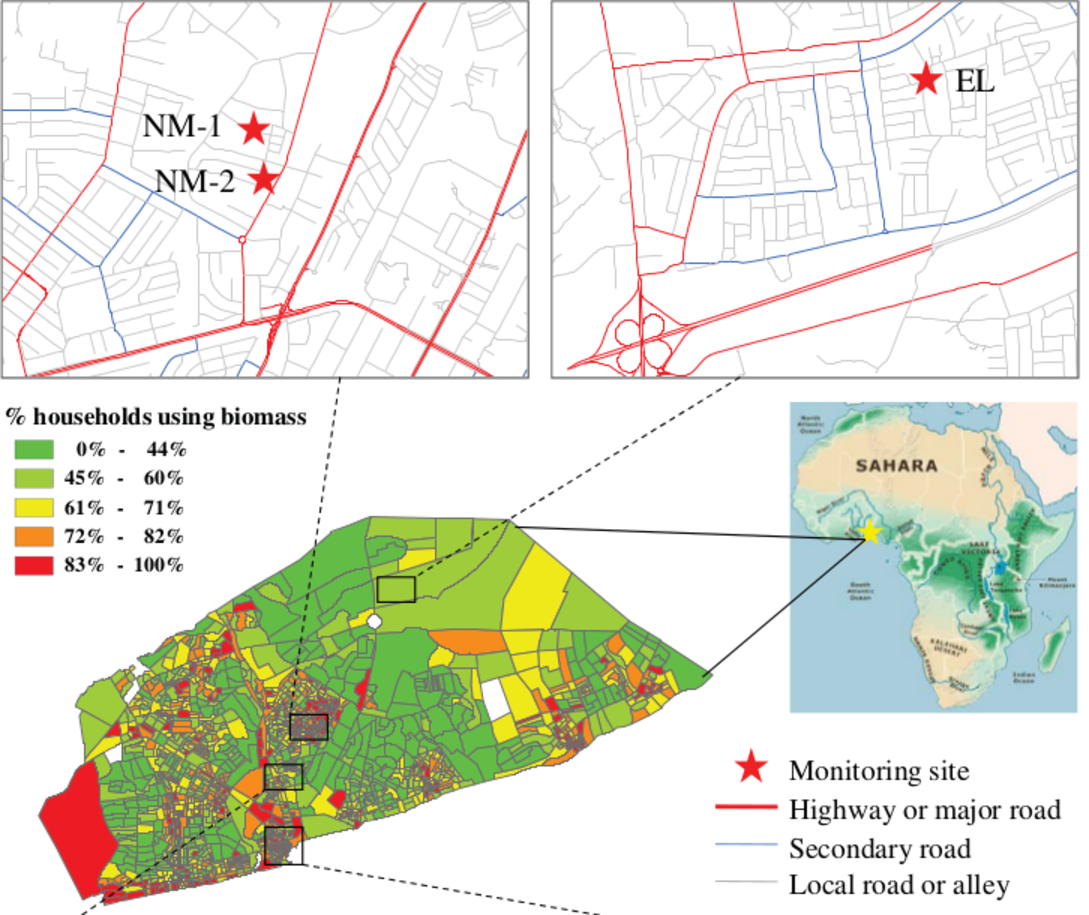
\includegraphics[width=0.7\textwidth]{../inputs/images/zheng/nima_mapa.pdf}
  \caption{Localização dos dois pontos de amostragem de Nima \label{fig:nima}}
\end{center}
\end{figure}

A coleta foi diária, mas houve dias sem medidas devido a falta de eletricidade,
problemas no amostrador, filtros danificados, ausência do operador, entre outros. 

Concentrações dos poluentes variam ao longo do dia na atmosfera
e quanto menor o tempo de amostragem, se obtém melhor resolução 
para identificação das fontes. Porém, amostras com concentrações menores, 
são mais difíceis de se medir devido ao limite de detecção dos equipamentos
\citep{calzolai2015}. 12 ou menos horas de amostragem permitiria captar 
a variabilidade das fontes de Acra (por ser uma região muito poluída).
Mas, o tempo de amostragem foi de 48 horas, e foi definido antes da 
entrada \textbf{USP} no projeto.

As amostras  foram coletadas em filtro de Teflon do tipo 
\textbf{PTFE} de 37 $mm$ de diâmetro, com orifícios de 0,2 $\mu m$ de diâmetro. 

%TODO: qual método foi utilizado para medir a área?
A área de deposição nos filtros foi de $7,32 (\pm 0,366) cm^2$ .

Impactadores são responsáveis pela coleta e classificação 
do material particulado, utilizando-se para tal a inercia das
partículas.
Para $MP_{10}$ utilizou-se impactador Harvard com $D_{50}$ de $10 \mu m$ 
com fluxo de $10,0 L/min$ \citep{marple1987}. 

Nas medidas de $MP_{2,5}$, também utilizou-se impactador Harvard, 
mas com $D_{50}$ de $2,5 \mu m$ acoplado com um \textbf{inlet} 
responsável fazer a filtragem de $MP_{2,5}$.

Os volumes amostrados foram medidos por um integrador de volume
com 5\% de incerteza.

Filtros brancos de campo e laboratórios foram separados para avaliar 
possíveis contaminações no tranporte e manipulação das amostras. 

O laboratório da \textbf{Harvard School of Public Health} foi
utilizado para pesagem das amostras.

Os filtros foram pesados antes e depois da amostragem, usando uma balança 
microanalítica \textbf{(Mettler Toledo MT5)} com precisão de $1 \mu g$, 
seguindo procedimentos padrões de controle de umidade ($39 \pm 2 \%$), 
temperatura ($20,5 \pm 0,2 ^{\circ} C$) e eliminação de cargas eletrostáticas 
(fonte de polônio). 
Cada medida de pesagem foi realizada duas vezes e o valor final foi a média das 
duas medidas. 
